\documentclass[12pt]{article}
\usepackage{../../template}
\title{Lecture 8}
\author{niceguy}
\begin{document}
\maketitle

\section{Transient Response}

The response of a pulse can be thought of as the superposition of 2 step functions. This applies to the transient response also.

\section{Bounce Diagram}

\begin{figure}[h]
    \begin{center}
        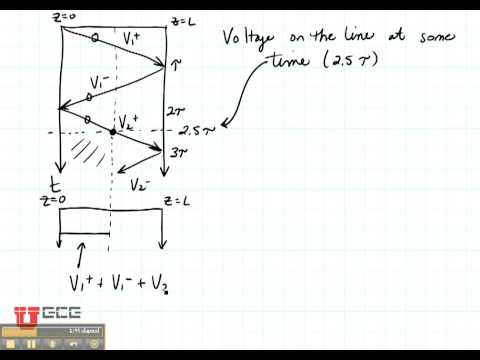
\includegraphics[scale=0.5]{bounce.jpg}
    \end{center}
\end{figure}

The Bounce Diagram shows the pulses travelling along length and time. Drawing a vertical line at $z = z_0$, we can observe voltage against time. at every time $t_i$ where the line intersects with bounce $v_i$, voltage changes by $v_i$. Drawing a horizontal line instead, we can see, at a certain time $t=t_0$, voltage distribution over the line. At $z = 0$, the voltage is the sum of all voltages above it. The wavefront is located where the horizontal line intersects with $v_i$, where there is a corresponding step (sign depends on direction of bounce). \\
At an arbitrary point, if we apply superposition to transform the step function into a pulse, graphical methods show that this results in discrete pulses with decreasing magnitudes (width of pulses and space between successive pulses both nonzero). 

\begin{ex}
    Consider a transmission line with $v_g = 10\unit{V}, R_g = 100\unit{\Omega}, R_L = 25\unit{\Omega}, l = 0.1\unit{m}, v_p = 3 \times 10^8 \unit{m.s^{-1}}, Z_0 = 50\unit{\Omega}$. Find $V(z = \frac{l}{2,} t), V(z, t = \frac{T}{2}), V(z, t = T)$. \\
    First we find $\Gamma_L$ and $\Gamma_g$.
    $$\Gamma_L = \frac{R_L - R_0}{R_L + R_0} = \frac{25-50}{25+50} = -\frac{1}{3}$$
    $$\Gamma_g = \frac{R_g - R_0}{R_g + R_0} = \frac{100-50}{100+50} = \frac{1}{3}$$
    Then
    $$v_1^+ = 10 \times \frac{50}{50 + 100} = \frac{10}{3}\unit{V}$$
    $$v_1^- = \Gamma_Lv_1^+ = -\frac{10}{9}\unit{V}$$
    $$v_2^+ = \Gamma_gv_1^- = -\frac{10}{27}\unit{V}$$
    $$v_2^- = \frac{10}{81}$$
    Using these values it then becomes trivial to find the graphs.
\end{ex}

\end{document}
